\chapter{Win32 API (24)}

Zadania z tej grupy mają zapoznać słuchaczy z fundamentami architektury systemów Windows: oknami, uchwytami i przepływem komunikatów.
Poznajemy także kilka wybranych podsystemów Win32 i interfejs ich programowania (Win32API {\em Application Programming Interface}). 
Współcześnie interfejsu tego prawie nie używa się do wytwarzania nowych aplikacji, co nie zmienia faktu, że nadal stanowi on fundament całego systemu operacyjnego.
Poznanie Win32 to więc tak naprawdę zrozumienie jak działają systemy operacyjne z rodziny Windows.

Rozwiązanie zadań w tym rozdziale polega na napisaniu programów w
języku C, przy czym w programach wolno korzystać wyłącznie z funkcji bibliotek standardowych
C oraz Win32 API. Tam gdzie to możliwe należy wybierać funkcje z Win32API zamiast ich odpowiedników
z C (na przykład przy obsłudze systemu plików czy allokacji pamięci). 

\section{Elementy interfejsu użytkownika (8)}

\subsection{Wykresy funkcji (1)} 

      Napisać program, który tworzy okno i w jego obszarze roboczym rysuje wykresy funkcji $f(x) = |x|$ i 
\label{wykres_z_osiami}	  
      $f(x) = x^2$ (z osiami). Oba wykresy powinny być narysowane różnymi kolorami i różnymi stylami pędzli.
      
      Wykresy powinny automatycznie dopasowywać się do nowych rozmiarów okna podczas skalowania okna.
      
      [{\bf 1p}]

\subsection{Poruszające się kółko (1)} 

      Napisać program, który w obszarze roboczym okna pokaże poruszające się i odbijające się od ramki okna kółko. 
\label{poruszajace_kolko}
      
      Kółko powinno poprawnie reagować na skalowanie rozmiarów okna przez użytkownika.
      
      [{\bf 1p}]

\subsection{Okno dialogowe (2)} 
      
      Napisać program, który odtworzy następujący wygląd okna z rysunku \ref{r1}.
\label{okno_dialogowe}

	\begin{figure}
	\begin{center}
	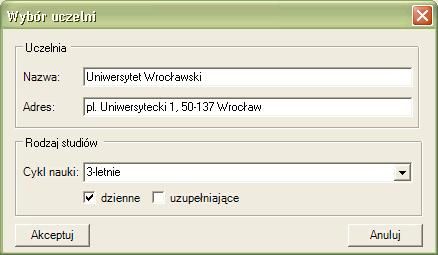
\includegraphics[width=0.75\textwidth]{z1_01}
	\end{center}
	\caption{Wygląd okna do zadania [\ref{okno_dialogowe}]}
	\label{r1}
	\end{figure}

      Okno zawiera dwie ramki grupujące ({\em Group Box}). Pierwsza ramka zawiera dwa pola tekstowe
      ({\em Edit Box}), druga zawiera pole wyboru ({\em Combo Box}) oraz dwa przyciski stanu ({\em Check Box}).

      Lista rozwijalna pola wyboru powinna być wypełniona przykładowymi nazwami.

      Po wybraniu przez użytkownika przycisku {\bf Akceptuj}, wybór powinien zostać zaprezentowany w oknie
      informacyjnym (rysunek \ref{r2}).

      	\begin{figure}
	\begin{center}
	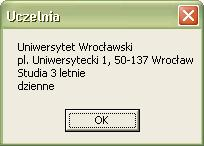
\includegraphics[width=0.25\textwidth]{z1_02}
	\end{center}
	\caption{Informacja dla użytkownika do zadania [\ref{okno_dialogowe}]}
	\label{r2}
	\end{figure}

      Naciśnięcie przycisku {\bf Anuluj} powinno zakończyć program.
      
      {\em Uwaga! Formanty potomne należy inicjować bezpośrednio przez {\tt CreateWindow}. Komunikat w oknie informacyjnym zależy oczywiście od
      danych wprowadzonych przez użytkownika na formularzu głównym}.
      
      [{\bf 2p}]

\subsection{Szablon okna dialogowego (2)} 
      
      Powtórzyć funkcjonalność programu z zadania [\ref{okno_dialogowe}] używając tym razem 
\label{szablon_okna}	  
	  edytora zasobów i wbudowanej w niego wizualnego funkcji wizualnej edycji szablonu okna do zbudowania interfejsu użytkownika. 
	  
      {\em Uwaga! W przypadku tworzenia okna z szablonu zapisanego w zasobach, zmiast {\tt RegisterClass}, {\tt CreateWindow} i jawnej pętli obsługi komunikatów użyć funkcji {\tt DialogBox}}.

      [{\bf 2p}]

\subsection{Wybrane składniki {\tt Common Controls} (2)}

      Napisać program, który zademonstruje działanie trzech wybranych komponentów biblioteki formantów Common Controls
\label{common_controls}	  
      (ListView, TreeView, Progress Bar, Status Bar, Tool Bar, itd.). Demonstracja ma polegać
      na obsłudze kilku wybranych właściwości komponentów (na przykład wypełnieniu ListView kilkoma
      elementami, zmianie wartości i stylu Progress Bara itp.). 
      
      [{\bf 2p}]
            

\section{Inne podsystemy Windows (10)}

\subsection{Plik tekstowy na pulpicie, pow�oka (1)}

      Napisa� program, kt�ry na pulpicie bie��cego zalogowanego u�ytkownika umie�ci
\label{powloka}	  
      plik tekstowy z bie��c� dat� systemow�. Nast�pnie plik ten skieruje do wydruku.

      Do pobrania nazwy foldera u�y� funkcji {\bf SHGetFolderPath}. Do skierowania dokumentu do wydruku
	  u�y� funkcji sterujacej pow�ok� {\bf ShellExecute}.
      
      [{\bf 1p}]

\subsection{Rozmiar okna w rejestrze (2)}

      Napisa� okienkowy program, kt�ry zapami�ta w rejestrze systemu rozmiary swojego okna.
\label{okno_w_rejestrze}	  
      Rozmiary te powinny by� odtwarzane przy ka�dym uruchomieniu i zapami�tywane przy
      zamykaniu okna programu.
      
      Zaprojektowa� format zapisu do rejestru. Zapisywa� pod kluczem:
      
      HKEY\_CURRENT\_USER$\backslash$Software$\backslash$Programowanie pod Windows$\backslash$...	  
	  
      [{\bf 2p}]

\subsection{Problem golibrody (2)}

      Napisa� konsolowy program, kt�ry rozwi�zuje klasyczny problem golibrody lub problem "palaczy tytoniu" 
\label{golibroda}	  
       za pomoc� jeden z metod synchronizacji w�tk�w udost�pnianej przez Win32:
	   \begin{itemize}
	   \item muteksy
	   \item semafory
	   \item zdarzenia
	   \end{itemize}

      [{\bf 2p}]
      
\subsection{Internet Explorer jako host dla aplikacji okienkowych (2)}

      Napisa� aplikacj� HTA (HTML Application), kt�ra w g��wnym oknie programu pozwoli wpisa�
\label{aplikacja_hta}	  
      imi�, nazwisko i dat� urodzenia, a po naci�ni�ciu przycisku "OK" zapisze
      dane do wybranego przez u�ytkownika pliku tekstowego.
      
      Dlaczego, mimo budowania interfejsu w HTML ta technologia nie
      mo�e by� u�yta do budowy aplikacji internetowych?
      
      [{\bf 2p}] 
      
\subsection{Informacje o systemie (3)}

      Napisa� program do diagnozowania komponent�w komputera i systemu operacyjnego. 
\label{informacje_o_systemie}	  
      Raport powinien obejmowa� m.in.
      \begin{itemize}
      \item Model procesora oraz cz�stotliwo�� taktowania 
      \item Ilo�� pami�ci operacyjnej (wolnej, ca�ej)
      \item Wersj� systemu operacyjnego wraz z wersj� uaktualnienia 
      \item Nazw� sieciow� komputera i nazw� aktualnie zalogowanego u�ytkownika
      \item Ustawienia rozdzielczo�ci i g��bi kolor�w pulpitu
      \item List� drukarek pod��czonych do systemu
      \item Obecno�� i numery wersji
            \begin{itemize}
            \item platformy .NET
            \item Internet Explorera
            \item Microsoft Worda
            \end{itemize}
      \end{itemize} 

      [{\bf 3p}] 
      

\section{Component Object Model (6)}

Rozwi�zanie zada� w tym rozdziale polega na napisaniu program�w w
j�zyku C++, korzystaj�c z wbudowanych w Visual Studio szablon�w projekt�w bibliotek COM.

\subsection {Automaryzacja Word (2)}

      Napisa� w C/C++ aplikacj� konsoli, kt�ra za po�rednictwem podsystemu COM otworzy now� instancj� aplikacji MS Word, a w niej otworzy
\label{com_client}	  
	  nowy dokument,
      do kt�rego wstawi tekst "Programowanie pod Windows". Nast�pnie dokument zostanie zapisany na dysku pod nazw� "ppw.doc".
      
	  Wzorowa� si� na poni�szym kodzie:
\begin{scriptsize}	  
\begin{verbatim}
void main()
{
	CoInitialize(NULL);

	CLSID clsid;
	OLECHAR wb[] = L"Word.Application";
	CLSIDFromProgID(wb, &clsid);

	OLECHAR pszCLSID[39];
	StringFromGUID2(clsid, pszCLSID, 39);
	
	char buffer[39];
	wsprintf(buffer, "%S", pszCLSID);
	cout << "CLSID: " << buffer << endl;

	IDispatch* pDispatch;
	CoCreateInstance(clsid, NULL, CLSCTX_SERVER, IID_IDispatch, (void**)&pDispatch);

	DISPID dispid;
	OLECHAR* szMember = L"Visible";

	HRESULT hr = 
	   pDispatch->GetIDsOfNames(IID_NULL, &szMember, 1, LOCALE_SYSTEM_DEFAULT, &dispid);
	if(FAILED(hr))
	    cout << "GetIDsOfNames failed" << endl;
	    cout << "DispID of Visible = " << dispid << endl;

	VARIANTARG test = { VT_BOOL, 0, 0, 0, VARIANT_TRUE };
	DISPID dispidnamed = DISPID_PROPERTYPUT;
	DISPPARAMS param = { &test, &dispidnamed, 1, 1 };

	hr = pDispatch->Invoke(dispid, IID_NULL, LOCALE_SYSTEM_DEFAULT,
		DISPATCH_PROPERTYPUT, &param, NULL, NULL, NULL);
	if(FAILED(hr))
		cout << "Invoke failed" << endl;

	pDispatch->Release();
	CoUninitialize();
}
\end{verbatim}
\end{scriptsize}
	  
      [{\bf 2p}]

\subsection {Serwer COM (3)}

      Przygotowa� w C++ serwer COM, udost�pniaj�cy funkcj� {\tt int IsPrime( int n )} umo�liwiaj�c� sprawdzenie, czy podana liczba jest liczb� 
\label{com_server}	  	  
	  pierwsz�. Funkcja powinna zwraca�
      zero dla argumentu b�d�cego liczb� z�o�on� i dowoln� niezerow� warto�� dla argumentu b�d�cego liczb� pierwsz�.

      {\em Wskaz�wka: w Visual Studio nale�y rozpocz�� od projektu C++/ATL Project. 
      Nast�pnie w widoku Class View u�y� funkcji Add/ATL COM+ 1.0 Component. 
      Dalsze kroki post�powania zmierzaj�cego do zbudowania serwera COM zostan�
      zaprezentowane na wyk�adzie.}

      [{\bf 3p}]

\subsection {Klient COM w VBA (1)}

      Napisa� w Visual Basic for Applications (j�zyk skryptowy Microsoft Office) funkcj� wykorzystuj�c� serwer COM z poprzedniego zadania. 
	  Rozwi�zanie nie musi posiada� �adnego interfejsu u�ytkownika do wygodnego wprowadzania argumentu funkcji.

      [{\bf 1p}]

	  
